\documentclass[tikz]{standalone}
\begin{document}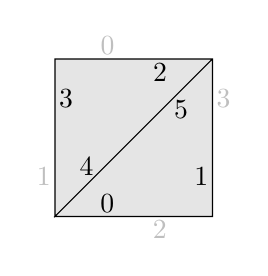
\begin{tikzpicture}[scale=2]
\fill[gray!20] (0,0) rectangle (1,1);

\draw (0,0) --
    node[pos=0.333, above=-2] {0}
    node[pos=0.666, below=-2, gray!50] {2} (1,0)
 -- node[pos=0.25, left=-2] {1}
    node[pos=0.75, right=-2, gray!50] {3} (1,1)
 -- node[pos=0.333, below=-2] {2}
    node[pos=0.666, above=-2, gray!50] {0} (0,1)
 -- node[pos=0.25, right=-2] {3}
    node[pos=0.75, left=-2, gray!50] {1} (0,0)
 -- node[pos=0.2, above] {4}
    node[pos=0.8, below] {5} (1,1)
 -- cycle;
 
\end{tikzpicture}\end{document}
